\section{Passo 5 — Triagem, etapa 1: a família trata do tema?}
\label{sec:passo5}

\subsection*{Objetivo}
Decidir, família por família, se o documento mantém relação com o tema e o contexto definidos no
estudo. É a etapa que separa volume de corpus.

\begin{figure}[H]
\centering
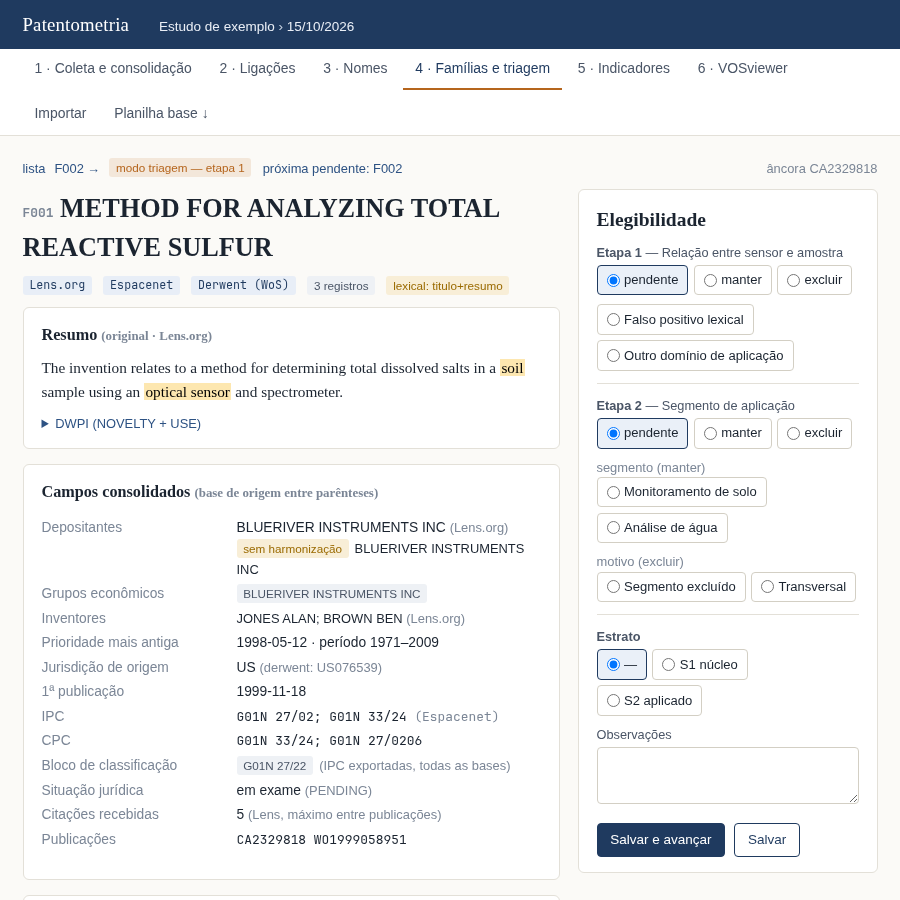
\includegraphics[width=0.78\linewidth]{img/08_triagem_topo.png}
\caption{Ficha de triagem. À esquerda, título e resumo com os termos dos blocos destacados e os dados
consolidados da família; à direita, o painel de decisão.}
\label{fig:triagem1}
\end{figure}

\subsection*{O que fazer}
\begin{enumerate}
\item Na rodada, clique em \textbf{Triar} (etapa 1). A aplicação abre a primeira família pendente.
\item Leia título e resumo com os destaques. Confira depositantes, prioridade e classificações.
\item Marque \textbf{Manter} ou \textbf{Excluir}. Ao excluir, escolha o motivo na lista.
\item Use \textbf{Salvar e próxima} para registrar e seguir. Repita até não haver pendentes.
\end{enumerate}

\subsection*{Como interpretar}
O destaque mostra onde os termos dos blocos aparecem. Um destaque no título é mais forte que um
destaque no resumo; um destaque isolado, sem relação semântica, é o típico falso positivo lexical.

A decisão é da \emph{família}, não do documento: o objetivo é não contar a mesma invenção duas vezes.
Três leituras ajudam a manter consistência:

\begin{itemize}
\item \textbf{Relação com o tema}: o tema é o objeto da invenção ou apenas uma palavra no texto?
\item \textbf{Relação com o contexto}: a aplicação declarada está no contexto do estudo?
\item \textbf{Evidência suficiente}: título e resumo bastam para decidir? Se não, use a ficha completa
      (Passo 9) antes de marcar.
\end{itemize}

\begin{nota}[O que ``manter'' significa]
Manter na etapa 1 não é incluir no corpus final: é admitir a família na etapa 2 (segmento) e na
classificação por estrato. A exclusão, ao contrário, é definitiva para esta rodada e alimenta os
motivos do PRISMA.
\end{nota}

\begin{alerta}[Erro comum]
Decidir pelo número de citações. Citação mede visibilidade na base, não aderência ao tema; uma família
muito citada pode ser justamente um falso positivo.
\end{alerta}

\subsection*{Checkpoint}
\marcador\; O contador de pendentes da etapa 1 chega a zero e o PRISMA passa a mostrar mantidas e
excluídas com seus motivos.
